%---------------------------------------------------
% Nombre: capitulo1.tex  
% 
% Texto del capitulo 1
%---------------------------------------------------

\chapter{Introducci�n}

En este documento encontramos el resultado final alcanzado durante el estudio del apartado de \textbf{miner�a de flujos de datos}, enmarcado dentro de la asignatura de `Miner�a de Series Temporales y Flujos de Datos' del m�ster en Ciencia de Datos de la Universidad de Granada. En este primer cap�tulo, veremos una introducci�n al problema a resolver as� como a los objetivos a alcanzar con esta pr�ctica y la organizaci�n del trabajo.

\section{Problema a resolver}
\label{problema}

El problema a resolver en esta pr�ctica se centrar� en la resoluci�n de ciertos problemas de clasificaci�n con flujos de datos, de manera tanto est�tica como din�mica as� como con cambio o sin cambio de contexto. Para resolver estos problemas, se propone el uso del software MOA \cite{moa} \cite{moa2} el cual usaremos con la l�nea de comandos o con la interfaz gr�fica que podemos ver en la figura \ref{moa}. 

\begin{figure}[h]
	\centering
		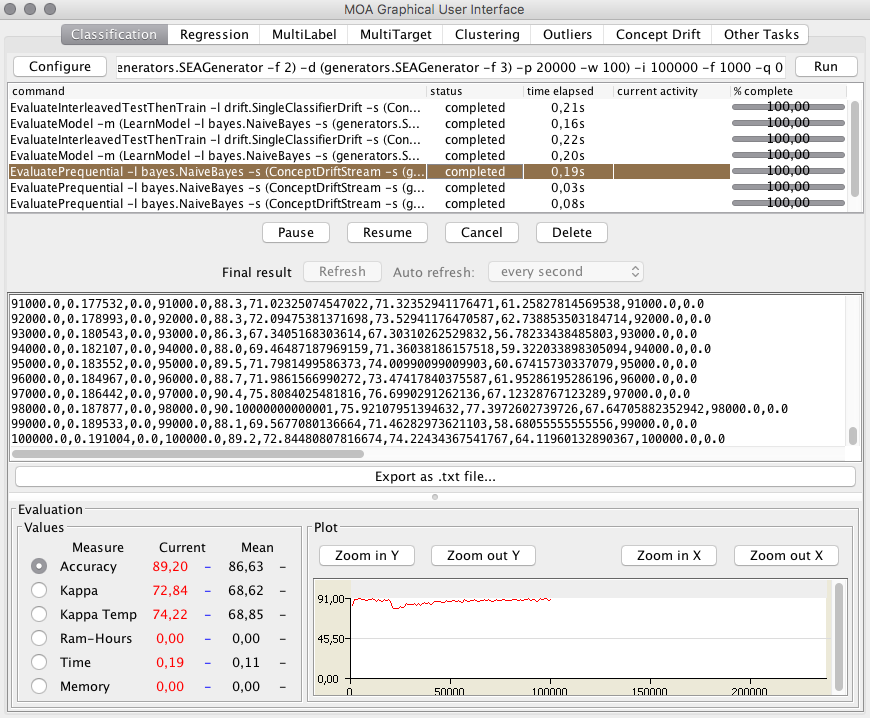
\includegraphics[scale=0.4]{./Capitulo1/imagenes/moa.png}
		\caption{Interfaz del software moa.}
	\label{moa}
\end{figure}


Los problemas a resolver ser�n:

\begin{enumerate}
\item Entrenamiento offline (estacionario) y evaluaci�n posterior.
\item Entrenamiento online.
\item Entrenamiento online en datos con concept drift.
\item Entrenamiento online en datos con concept drift, incluyendo mecanismos para olvidar instancias pasadas.
\item Entrenamiento online en datos con concept drift, incluyendo mecanismos para reinicializar modelos tras la detecci�n de cambios de concepto.
\end{enumerate}

Posteriormente a la soluci�n de estos problemas, se propone una discusi�n te�rica de los resultados, por lo que encontraremos la pr�ctica dividida en dos apartados, por un lado el te�rico ( cap�tulo \ref{teoria}) y por otro el pr�ctico (\ref{practica}).

\section{Objetivos}
\label{objetivos}

Los objetivos de esta pr�ctica ser�n:

\begin{itemize}
	\item Asentar y comprender la materia te�rica de la miner�a de flujo de datos vista durante el transcurso de la asignatura.
	\item Comprender el uso y formas de utilizaci�n del software MOA.  
	\item Asentar el conocimiento sobre test estad�sticos par comparaci�n de modelos.
	\item Elaboraci�n de una memoria donde se recojan todos los resultados de manera apropiada.
\end{itemize}

\section{Organizaci�n del trabajo} 

La organizaci�n del presente documento, se centra en detallar cada uno de los pasos seguidos durante el estudio y resoluci�n del problema planteado en esta introducci�n, tras la cual tendremos el contenido pr�ctico en el cap�tulo \ref{practica}  y el cual representa el grueso de esta memoria. Tras este cap�tulo encontramos el cap�tulo \ref{teoria} donde desde un punto de vista te�rico analizamos el concepto de \textbf{clasificaci�n} y \textbf{concept drift} en miner�a de flujo de datos. Finalizaremos la memoria con las conclusiones obtenidas en el transcurso de finalizaci�n de la misma en el cap�tulo \ref{conclusiones}. 
\clearpage
%---------------------------------------------------